\documentclass{article}\usepackage[]{graphicx}\usepackage[]{xcolor}
% maxwidth is the original width if it is less than linewidth
% otherwise use linewidth (to make sure the graphics do not exceed the margin)
\makeatletter
\def\maxwidth{ %
  \ifdim\Gin@nat@width>\linewidth
    \linewidth
  \else
    \Gin@nat@width
  \fi
}
\makeatother

\definecolor{fgcolor}{rgb}{0.345, 0.345, 0.345}
\newcommand{\hlnum}[1]{\textcolor[rgb]{0.686,0.059,0.569}{#1}}%
\newcommand{\hlstr}[1]{\textcolor[rgb]{0.192,0.494,0.8}{#1}}%
\newcommand{\hlcom}[1]{\textcolor[rgb]{0.678,0.584,0.686}{\textit{#1}}}%
\newcommand{\hlopt}[1]{\textcolor[rgb]{0,0,0}{#1}}%
\newcommand{\hlstd}[1]{\textcolor[rgb]{0.345,0.345,0.345}{#1}}%
\newcommand{\hlkwa}[1]{\textcolor[rgb]{0.161,0.373,0.58}{\textbf{#1}}}%
\newcommand{\hlkwb}[1]{\textcolor[rgb]{0.69,0.353,0.396}{#1}}%
\newcommand{\hlkwc}[1]{\textcolor[rgb]{0.333,0.667,0.333}{#1}}%
\newcommand{\hlkwd}[1]{\textcolor[rgb]{0.737,0.353,0.396}{\textbf{#1}}}%
\let\hlipl\hlkwb

\usepackage{framed}
\makeatletter
\newenvironment{kframe}{%
 \def\at@end@of@kframe{}%
 \ifinner\ifhmode%
  \def\at@end@of@kframe{\end{minipage}}%
  \begin{minipage}{\columnwidth}%
 \fi\fi%
 \def\FrameCommand##1{\hskip\@totalleftmargin \hskip-\fboxsep
 \colorbox{shadecolor}{##1}\hskip-\fboxsep
     % There is no \\@totalrightmargin, so:
     \hskip-\linewidth \hskip-\@totalleftmargin \hskip\columnwidth}%
 \MakeFramed {\advance\hsize-\width
   \@totalleftmargin\z@ \linewidth\hsize
   \@setminipage}}%
 {\par\unskip\endMakeFramed%
 \at@end@of@kframe}
\makeatother

\definecolor{shadecolor}{rgb}{.97, .97, .97}
\definecolor{messagecolor}{rgb}{0, 0, 0}
\definecolor{warningcolor}{rgb}{1, 0, 1}
\definecolor{errorcolor}{rgb}{1, 0, 0}
\newenvironment{knitrout}{}{} % an empty environment to be redefined in TeX

\usepackage{alltt}

\usepackage{tikz}
\usetikzlibrary{arrows}
\usetikzlibrary{positioning}
\usetikzlibrary{shapes.geometric}
%\usepackage{wrapfig}     % To wrap text around figures.
\PassOptionsToPackage{hyphens}{url}
% \usepackage[colorlinks=true,linkcolor=MyDarkBlue,
% citecolor=MyDarkBlue,filecolor=MyDarkBlue,urlcolor=MyDarkBlue]{hyperref}
\usepackage{hyperref}
\usepackage{doi}
\IfFileExists{upquote.sty}{\usepackage{upquote}}{}
\begin{document}  

\title{A Calvin Core 100 Introduction to Sustainability}
\author{Jeremy Van~Antwerp, Matthew Kuperus Heun}

\maketitle

In the long run, sustainability is one of the few things that matter at all.
Sustainability is a challenging problem, in part
because sustainability problems are complex and interconnected,
and because we operate with limited knowledge.
In sustainability, there is tremendous social (and sometimes economic) pressure
to continue to do things ``the way they've always been done.''

Figure~\ref{fig:venn_diagram} shows the three interrelated and overlapping
domains of sustainability:
\textbf{environmental sustainability},
\textbf{economic sustainability}, and
\textbf{social sustainability}.
Sustainability problems are complex and interconnected.
Environmental sustainability problems have social and economic aspects 
(that are generally more difficult to solve).
Likewise, economic and social sustainability problems are not limited to one domain;
typically, they include aspects of the other two domains as well.
Therefore (for example), pollution is an environmental problem, and a social problem, and an economic problem.
Likewise renewable energy. And land use. 
And all the other challenges humanity faces.

\begin{figure}
\centering

  % The next command tells RStudio to do "Compile PDF" on book.Rnw,
% instead of this chapter, thereby eliminating the need to switch back to book.Rnw 
% before making the book.
%!TEX root = ../../book.Rnw

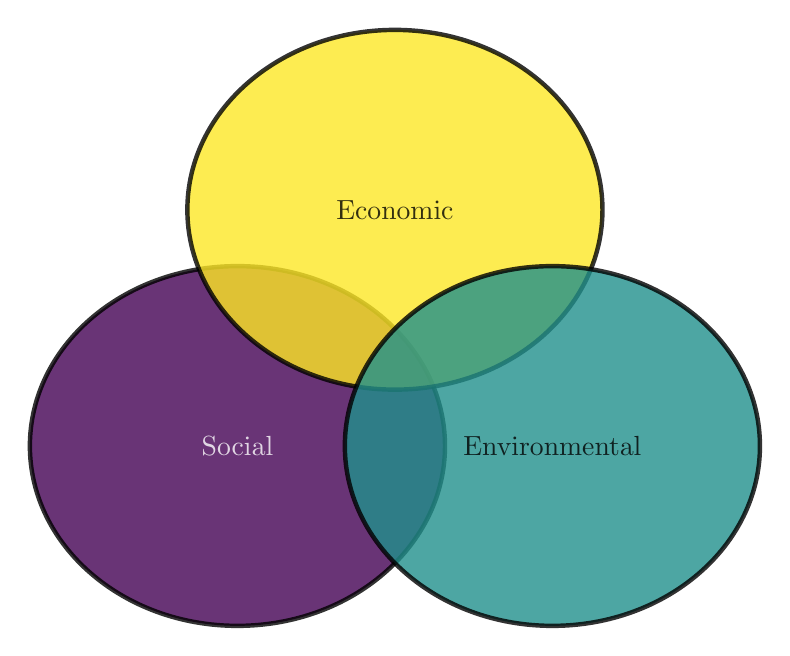
\begin{tikzpicture}
    \definecolor{my_purple}{HTML}{440154}
    \definecolor{my_yellow}{HTML}{FDE725}
    \definecolor{my_green}{HTML}{21908C}
    \tikzstyle{every node}=[ultra thick, ellipse, 
                            minimum width = 150pt,
                            minimum height = 130pt]
    \node[ellipse, draw, fill = my_purple, opacity = 0.8, align = left, text = white] (social) at (-2,0) {Social};
    \node[ellipse, draw, fill = my_yellow, opacity = 0.8, align = center] (economic) at (0,3) {Economic};
    \node[ellipse, draw, fill = my_green, opacity = 0.8, align = right] (environmental) at (2,0) {Environmental};
\end{tikzpicture}


  \caption[Three aspects of sustainability]
          {The three aspects of sustainability.
           Sustainability is often visualized as three overlapping ellipses:
           economic sustainability,
           environmental sustainability, and
           social sustainability.
           The intersecting area represents fully sustainable living.
           Environmental sustainability
           refers to the \textbf{ecosystem} and its supporting services.
           Economic sustainability refers to human systems for creating 
           and accounting for wealth.
           Social sustainability refers to traditions and systems of human society.
           The layering in this figure represents coverage in this book.
           We focus on environmental and
           economic sustainability.
           Social sustainability is vitally important, so it forms the backdrop
           for much of the discussion herein.}
\label{fig:venn_diagram}
\end{figure}


Sustainability is challenging for two additional reasons.
First, it may seem that the changes required to achieve sustainability are so
massively overwhelming that they shouldn't even be addressed.
Second, it may seem like the consequences of not becoming sustainable are so far
in the future that there is neither urgency nor immediate payback.
However, neither of these views is true.
Current news headlines indicate that we are already
experiencing the effects of not being sustainable, in all
sustainability domains---environmentally, economically, and socially.
There are many reasonable and simple things that can be done to improve our
sustainability in the near term.
The deep changes needed for long-term sustainability are urgently needed precisely because
they are long-term investments.
The sooner we begin making those investments, the sooner we'll begin reaping the
rewards and the greater those rewards will be.

Because the choices and paths to sustainability are filled with 
value judgments and moral choices, 
navigating tradeoffs is a key to sustainability.



``Sustainability'' is a crucial concept.
If humanity is not living sustainably, 
we will either cease to exist as a species or (at least) 
experience drastic reductions in our population and/or standard of living.
So, what is sustainability and how do we tell if we're living sustainably?
There are many definitions of sustainability.
To the novice, many definitions may seem to indicate lack of agreement.
However, sustainability is almost a self-defining concept.
Different answers indicate different assumptions, different priorities, 
and different boundaries (that is, what system is being considered).

When considering the meaning of sustainability, 
the two most important questions are
``sustaining what?'' and ``for how long?''
The second of these questions is perhaps easier to answer.
Although humans seem to have inherent cognitive difficulties in planning for
time scales significantly longer than the human lifespan,
\textbf{strong sustainability} is achieved only if the answer is
``indefinitely'' or ``forever.''
Our current sustainability crisis has been thousands of years in the making~\cite{Sanderman2017}
and will likely require millions of years to recover~\cite{Davis11262}.
A \textbf{weak sustainability} criterion is sustainability over a long
(by human standards) time frame, perhaps 50 years, 
which is on the order of one human adulthood.%
% \footnote{
%   Our criteria for strong\index{strong sustainability} and weak sustainability\index{weak sustainability} are physical and
%   follow \citet{Graedel:2010ab}.
%   Other definitions for weak\index{weak sustainability} and strong sustainability\index{strong sustainability} exist.
%   One approach to weak\index{weak sustainability} and strong\index{strong sustainability} sustainability is economic.
%   It defines strong sustainability\index{strong sustainability} as protecting natural capital\index{natural capital}
%   for a certain period of time
%   (equivalent to our weak sustainability\index{weak sustainability} definition 
%   if the time horizon for protecting natural capital\index{natural capital} is 50 years).
%   In the economic approach,
%   weak sustainability\index{weak sustainability} allows 
%   produced capital\index{produced capital}
%   to substitute for natural capital\index{natural capital}
%   across a period of time.
%   See \citet{Dietz:2007tu} for details.
% }
(Note that corporate time scales for decision making are even shorter,
often in the 5--20 year range.)

The narrowest answer for what needs sustaining is human life and society, which
\href{https://www.merriam-webster.com/dictionary/perforce}{perforce}
entails those \textbf{ecosystem services}
necessary for human health and wellbeing.
Beyond these basics, some people view the nonhuman world as having inherent 
worth or standing and, therefore, to be worth preserving.
For some people, the inclination for preservation is limited to those parts
of the nonhuman world that humans find appealing, like flowers and songbirds.
Other people would include even those parts of the nonhuman world that negatively
affect humanity, like smallpox.
Unfortunately, humans don’t know clearly what pieces of the ecosystem
are, in the long run, necessary for our survival and which aren’t.
For instance, could we survive in a world without dandelions?
Maybe.
On the other hand, dandelions might be necessary for other organisms we depend on.
Environmental science views the ecosystem in its entirety as a web, with all parts
depending on all other parts.
The ecosystem is not a collection of individual components with binary ``needed''/``not
needed'' classifications, but as a whole that exists on a continuum from ``fully functional''
to ``nonfunctional.''
The choices and paths to sustainability are bristling with value judgments and
moral choices about what to value and how much.
\href{https://en.wiktionary.org/wiki/concomitant}{Concomitant} with such choices
is a weighting of appropriate risks to the ecosystem and human society.
Different answers to these questions come from different \emph{a priori} assumptions and values.

The broadest definitions of sustainability
also include the products of human civilization.
For example, although they are great cultural and historical artifacts,
humanity could survive without the great pyramids of Giza.
On the other hand, we may not survive if we don’t give up coal-fired power plants.
(And, maybe many people would perish if the coal-fired power plants
were all suddenly switched off.)

With respect to Figure \ref{fig:venn_diagram}, environmental sustainability
considers biophysical and thermodynamic constraints and includes issues such as
pollution, resource depletion, habitat loss, and biodiversity.
Harvesting timber faster than it can grow is unsustainable.
Eventually, deforestation means that timber harvesting must stop because there
will be no more forest to harvest.
Depleting \textbf{mineral resources} is unsustainable.
Eventually, the minerals will be used up.
Pumping \textbf{aquifers} faster than they can regenerate is unsustainable.
Eventually, the aquifers will run dry.

Economic sustainability
involves questions of profit and loss, wealth management, and
macroeconomic policy.
A business that continually loses money is not sustainable.
Eventually, it will go out of business.

Social sustainability comprises human and 
civil rights,
suffering, and personal freedom.
A social group that continually loses members, for example, the Whig party, will
cease to be a group.
Often, a discussion about social sustainability 
includes things that should not be sustained but that, typically,
have persisted for a very long time, like poverty, class inequality, sexism,
slavery, and other civil injustices.



\end{document}
